\documentclass[aspectratio=169,12pt]{beamer}
\usepackage[utf8]{inputenc}
\usepackage{amsmath, amssymb}
\usepackage{booktabs}
\usepackage{colortbl}
\usepackage{hyperref}
\usepackage{makecell}
\usepackage{ragged2e}
\usepackage{bytefield}
\usepackage{tikz}
\usetikzlibrary{arrows.meta, positioning, shapes.geometric, calc, tikzmark, shapes.misc}
\usetheme{Madrid}

% Define custom ALU shape command
\newcommand{\drawALU}[1]{
    \node[inner sep=0] (ALU) at #1 {
        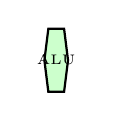
\begin{tikzpicture}[scale=0.5]
            % Trapezoid shape for ALU
            \coordinate (tl) at (-0.2, 0.8);
            \coordinate (tr) at (0.2, 0.8);
            \coordinate (ml) at (-0.3, 0);
            \coordinate (mr) at (0.3, 0);
            \coordinate (bl) at (-0.2, -0.8);
            \coordinate (br) at (0.2, -0.8);
            
            \fill[green!20] (tl) -- (tr) -- (mr) -- (br) -- (bl) -- (ml) -- cycle;
            \draw[thick] (tl) -- (tr) -- (mr) -- (br) -- (bl) -- (ml) -- cycle;
            
            \node[font=\tiny] at (0, 0) {ALU};
        \end{tikzpicture}
    };
}

% Define custom Adder shape command (similar to ALU but with +)
\newcommand{\drawAdder}[1]{
    \node[inner sep=0] (adder) at #1 {
        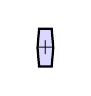
\begin{tikzpicture}[scale=0.4]
            \coordinate (tl) at (-0.2, 0.6);
            \coordinate (tr) at (0.2, 0.6);
            \coordinate (ml) at (-0.25, 0);
            \coordinate (mr) at (0.25, 0);
            \coordinate (bl) at (-0.2, -0.6);
            \coordinate (br) at (0.2, -0.6);
            
            \fill[blue!15] (tl) -- (tr) -- (mr) -- (br) -- (bl) -- (ml) -- cycle;
            \draw[thick] (tl) -- (tr) -- (mr) -- (br) -- (bl) -- (ml) -- cycle;
            
            \node[font=\scriptsize] at (0, 0) {+};
        \end{tikzpicture}
    };
}

% Define macro for placing adders in pipeline with configurable location and optional rotation
% Usage: \placeAdder{prefix}{x,y}[rotation angle]
\newcommand{\placeAdder}[3][0]{%
    \begin{scope}[shift={(#2)}, scale=0.8, rotate=#1]
        \coordinate (#3_adder) at (0,0);
        % Trapezoid coordinates
        \coordinate (toptopleft) at (0, 0.4);
        \coordinate (topbottomleft) at (0, 0.15);
        \coordinate (left) at (0.1, 0);
        \coordinate (bottomtopleft) at (0, -0.15);
        \coordinate (bottombottomleft) at (0, -0.4);
        \coordinate (topright) at (0.3, 0.2);
        \coordinate (bottomright) at (0.3, -0.2);
        
        % Draw the trapezoid
        \fill[blue!15] (toptopleft) -- (topbottomleft) -- (left) -- (bottomtopleft) -- (bottombottomleft) -- (bottomright) -- (topright) -- cycle;
        \draw[thick] (toptopleft) -- (topbottomleft) -- (left) -- (bottomtopleft) -- (bottombottomleft) -- (bottomright) -- (topright) -- cycle;
        
        % Add + text
        \node at (0.16, 0) {\tiny +};

        \coordinate (#3_adder_input1) at (0, 0.3);
        \coordinate (#3_adder_input2) at (0, -0.3);
        \coordinate (#3_adder_output) at (0.3, 0);
    \end{scope}
}

% Define macro for pipeline diagram
% Usage: \drawPipelineDiagram
\newcommand{\drawPipelineDiagram}{%
    \scalebox{0.85}{%
    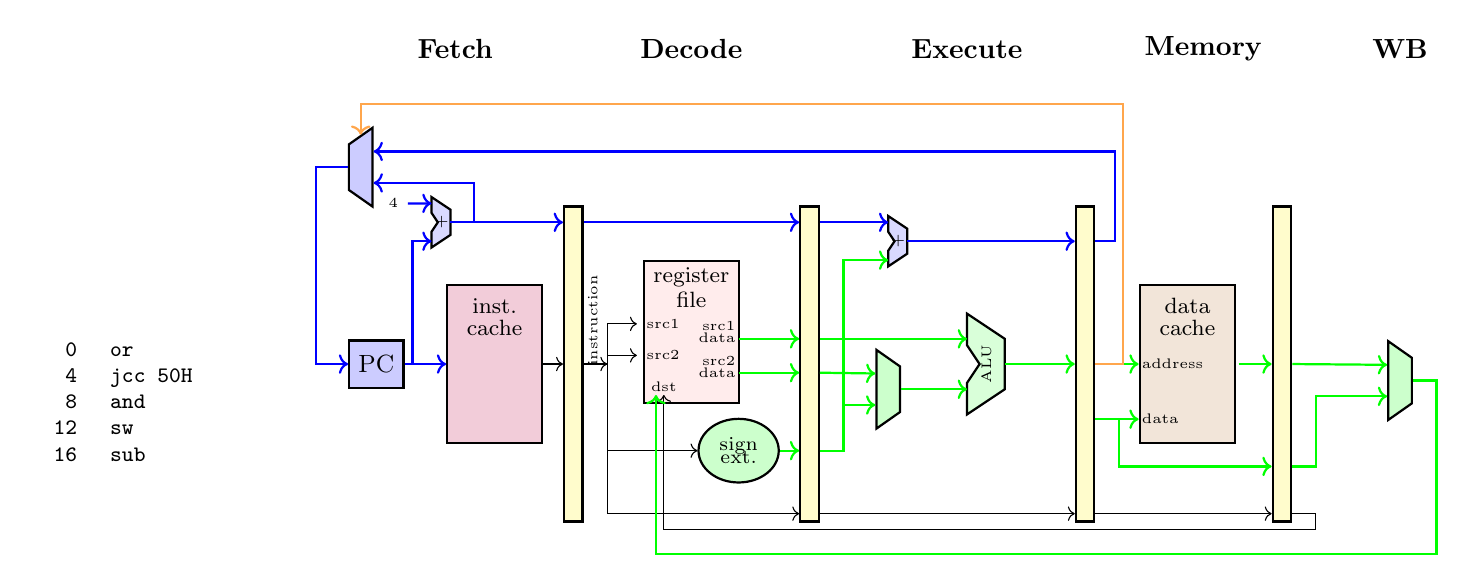
\begin{tikzpicture}[
        component/.style={draw, thick, minimum height=0.8cm},
        latch/.style={draw, thick, fill=yellow!20, minimum width=0.2cm, minimum height=4cm},
        stage/.style={font=\bfseries},
        label/.style={font=\tiny},
        port/.style={font=\tiny, inner sep=0.035cm}
    ]
        % Stage labels
        \node[stage] at (1.5,6) {Fetch};
        \node[stage] at (4.5,6) {Decode};
        \node[stage] at (8,6) {Execute};
        \node[stage] at (11,6) {Memory};
        \node[stage] at (13.5,6) {WB};
        
        % Pipeline latches
        \node[latch] (L1) at (3,2) {};
        \node[latch] (L2) at (6,2) {};
        \node[latch] (L3) at (9.5,2) {};
        \node[latch] (L4) at (12,2) {};
        
        % Fetch Stage
        % PC MUX (rotate=90: output on west)
        \placeMux[90]{0.3,4.5}{pc}{blue!20}

        \node[component, fill=blue!20, minimum width=0.6cm, minimum height=0.6cm] (PC) at (0.5,2) {\small PC};

        % ICache
        \node[component, fill=purple!20, minimum width=1.2cm, minimum height=2cm] (ICache) at (2,2) {};
        \node[align=center] at (2,2.6) {\footnotesize inst.\\[-0.14cm]\footnotesize cache};
 
        % PC adder - moved right
        \placeAdder{1.2,3.8}{fe}
        \node[left, font=\tiny] (four) at (0.9,4.04) {4};
        
        % Decode Stage
        \node[component, fill=pink!30, minimum width=1.2cm, minimum height=1.8cm] (RF) at (4.5,2.41) {};
        \node[align=center] at ([yshift=-0.35cm]RF.north) {\footnotesize register\\[-0.11cm]\footnotesize file};
        
        % Register file input ports (left side, inside the box)
        \node[port] (rf_src1) at ([xshift=-0.4cm, yshift=0.1cm]RF.center) {~src1};
        \node[port] (rf_src2) at ([xshift=-0.4cm, yshift=-0.3cm]RF.center) {~src2};
        \node[port] (rf_dst) at ([xshift=-0.35cm, yshift=-0.7cm]RF.center) {dst};
        
        % Register file selector coordinate (slightly left of dst)
        \coordinate (rf_selector) at ([xshift=-0.1cm]rf_dst.south);
        
        % Register file output ports (right side, aligned to right edge)
        \node[port, anchor=east] (rf_src1_data) at ([xshift=0.6cm, yshift=0.07cm]RF.center) {src1};
        \node[port, anchor=east] (rf_data1) at ([yshift=-0.15cm]rf_src1_data.east) {data};
        \node[port, anchor=east] (rf_src2_data) at ([xshift=0.6cm, yshift=-0.37cm]RF.center) {src2};
        \node[port, anchor=east] (rf_data2) at ([yshift=-0.15cm]rf_src2_data.east) {data};
        
        % Sign extension - moved slightly right
        \node[component, fill=green!20, ellipse, minimum width=0.4cm, minimum height=0.3cm, align=center] (SignExt) at (5.1,0.9) {
            \scriptsize sign\\[-0.25cm]\scriptsize ext.
        };
        
        % Execute Stage
        % Execute adder - positioned so input aligns with incoming connection
        \placeAdder{7,3.56}{ex}
        
        % Execute stage ALU source MUX (rotate=270: output on north, inputs on south)
        \placeMux[270]{7,1.68}{exe}{green!20}
        
        % ALU - positioned to align output with data cache address
        \begin{scope}[shift={(8,2)}, scale=0.8]
            \coordinate (ALU) at (0,0);
            % Trapezoid coordinates
            \coordinate (toptopleft) at (0, 0.8);
            \coordinate (topbottomleft) at (0, 0.3);
            \coordinate (left) at (0.2, 0);
            \coordinate (bottomtopleft) at (0, -0.3);
            \coordinate (bottombottomleft) at (0, -0.8);
            \coordinate (topright) at (0.6, 0.4);
            \coordinate (bottomright) at (0.6, -0.4);
            
            % Draw the trapezoid
            \fill[green!15] (toptopleft) -- (topbottomleft) -- (left) -- (bottomtopleft) -- (bottombottomleft) -- (bottomright) -- (topright) -- cycle;
            \draw[thick] (toptopleft) -- (topbottomleft) -- (left) -- (bottomtopleft) -- (bottombottomleft) -- (bottomright) -- (topright) -- cycle;
            
            % Add ALU text (rotated and smaller)
            \node[rotate=90, font=\tiny] at (0.31, 0) {ALU};

            \coordinate (alu_input1) at (0, 0.4);
            \coordinate (alu_input2) at (0, -0.4);
            \coordinate (alu_output) at (0.6, 0);
        \end{scope}
        
        % Memory Stage
        \node[component, fill=brown!20, minimum width=1.2cm, minimum height=2cm] (DCache) at (10.8,2) {};
        \node[align=center] at (10.8,2.6) {\footnotesize data\\[-0.14cm]\footnotesize cache};

        % Data Cache ports (aligned to left side of box)
        \node[port, anchor=west] (dc_addr) at ([xshift=-0.62cm, yshift=0cm]DCache.center) {address};
        \node[port, anchor=west] (dc_data) at ([xshift=-0.62cm, yshift=-0.7cm]DCache.center) {data};

        % DCache output port
        \node[port, anchor=east] (dc_data_out) at ([xshift=0.65cm, yshift=0cm]DCache.center){};
        
        % Write Back Stage MUX (rotate=-90: output on east, inputs on north/south)
        \placeMux[270]{13.5,1.79}{wb}{green!20}
        
        % Main data path connections
        \draw[blue, thick, ->] (four) -- (fe_adder_input1);
        \draw[blue, thick, ->] (pcmux_out) -- ++(-0.4,0) |- (PC.west);
        \draw[blue, thick, ->] (PC.east) -- (ICache);
        \draw[blue, thick, ->] (PC.east) -- ++(0.1,0) |- (fe_adder_input2);
        \draw[->] (ICache) -- (L1);

        \draw[blue, thick, ->] (fe_adder_output) -- (fe_adder_output -| L1.west);
        \draw[blue, thick, ->] (fe_adder_output) -- ++(0.3,0) |- (pcmux_in1);
        \draw[blue, thick, ->] (fe_adder_output -| L1.east) -- (fe_adder_output -| L2.west);
        \draw[blue, thick, ->] (fe_adder_output -| L2.east) -- ++(0.3,0) |- (ex_adder_input1);
        
        % From L1 to Register File inputs
        \draw[->] (L1.east) -- ++(0.3,0) |- (rf_src1.west);
        \draw[->] (L1.east) -- ++(0.3,0) |- (rf_src2.west);
        \draw[->] (L1.east) -- ++(0.3,0) |- (SignExt.west);

        \draw[->] (L1.east) -- ++(0.3,0) |- ([yshift=-0.8cm]SignExt -| L2.west);
        \draw[->] ([yshift=-0.8cm]SignExt -| L2.east) -- ([yshift=-0.8cm]SignExt -| L3.west);
        \draw[->] ([yshift=-0.8cm]SignExt -| L3.east) -- ([yshift=-0.8cm]SignExt -| L4.west);
        \draw[->] ([yshift=-0.8cm]SignExt -| L4.east) -- ++(0.3, 0) -- ++(0, -0.2) -| (rf_dst.south);

        % From L1 for "instruction" title
        \draw[->] (ICache -| L1.east) -- ++(0.3,0) node[yshift=0.55cm,rotate=90,above] {\tiny{}instruction}; 

        % From Register File outputs to L2
        \draw[green, thick, ->] ([yshift=-0.01cm]rf_data1.east) -- ([yshift=-0.01cm]rf_data1.east -| L2.west);
        \draw[green, thick, ->] (rf_data2.east) -- (rf_data2.east -| L2.west);
        \draw[green, thick, ->] (SignExt.east) -- (SignExt.east -| L2.west);
        
        % From L2 to Execute components
        \draw[green, thick, ->] ([yshift=-0.01cm]rf_data1.east -| L2.east) -- ++(0.2,0) |- (alu_input1);
        \draw[green, thick, ->] (rf_data2.east -| L2.east) -- (exemux_in1);
        \draw[green, thick, ->] (SignExt.east -| L2.east) -- ++(0.3,0) |- (exemux_in2);
        \draw[green, thick, ->] (SignExt.east -| L2.east) -- ++(0.3,0) |- (ex_adder_input2);
        
        % MUX to ALU
        \draw[green, thick, ->] (exemux_out) -- ++(0.3,0) |- (alu_input2);
        
        % ALU and adder to L3
        \draw[green, thick, ->] (alu_output) -- (L3.west |- alu_output);
        \draw[blue, thick, ->] (ex_adder_output) -- (L3.west |- ex_adder_output);
        \draw[blue, thick, ->] (L3.east |- ex_adder_output) -- ++(0.25,0) |- (pcmux_in2);
        
        % L3 to Memory and from
        \draw[green, thick, ->] (alu_output -| L3.east) -- (dc_addr.west);
        \draw[green, thick, ->] (dc_data.east -| L3.east) -- (dc_data.west);
        \draw[green, thick, ->] (dc_data.east -| L3.east) -- ++(0.3,0) |- ([yshift=-1.3cm]L4.west);
        \draw[green, thick, ->] (dc_data_out) -- (dc_data_out -| L4.west);
        
        % L4 to WB mux - ALU result and memory data
        \draw[green, thick, ->] (alu_output -| L4.east) -- (wbmux_in1);
        \draw[green, thick, ->] ([yshift=-1.3cm]L4.east) -- ++(0.3,0) |- (wbmux_in2);
        
        % Write back path from mux output
        \draw[green, thick, ->] (wbmux_out) -- ++(0.3,0) -- ++(0,-2.2) -| (rf_selector);
        
        % PC MUX inputs: branch target from L3, branch from L2, and PC+4
        \draw[orange!70, thick, ->] (alu_output -| L3.east) -- ++(0.35,0) -- ++(0,3.3) -| (pcmux_selectorup);
        
        % Code on the left
        \node[anchor=east, font=\footnotesize\ttfamily] at (-1.5,1.5) {
            \begin{tabular}{rl}
                0 & or\\
                4 & jcc 50H\\
                8 & and\\
                12 & sw\\
                16 & sub
            \end{tabular}
        };
    \end{tikzpicture}
    }%
}

% Define macro for placing MUX with configurable location, rotation, and fill color
% Usage: \placeMux[rotation]{x,y}{prefix}{fill color}
% rotation: angle in degrees (default 0)
% x,y: position
% prefix: name prefix for coordinates
% fill color: color for the mux (e.g., blue!20)
\newcommand{\placeMux}[4][0]{%
    \node[trapezium, trapezium left angle=70, trapezium right angle=70,
          trapezium stretches=true, minimum height=0.3cm, minimum width=1cm,
          draw, thick, fill=#4, rotate=#1] (#3mux) at (#2) {};
    
    % Define input/output coordinates based on rotation only
    % For trapezoid: unrotated has narrow left, wide right
    % Inputs should be on the wide side, output on narrow side
    \ifnum#1=90
        % Rotation 90: narrow side moves to bottom, wide side to top
        % So output should be on south (narrow), inputs on north (wide)
        \coordinate (#3mux_in1) at ([yshift=-0.2cm]#3mux.south);
        \coordinate (#3mux_in2) at ([yshift=0.2cm]#3mux.south);
        \coordinate (#3mux_out) at (#3mux.north);
        % Selector positions
        \coordinate (#3mux_selectorup) at (#3mux.east);
        \coordinate (#3mux_selectordown) at (#3mux.west);
    \else\ifnum#1=180
        % Rotation 180: narrow side moves to right, wide side to left
        % So output on east (narrow), inputs on west (wide)
        \coordinate (#3mux_in1) at ([yshift=0.2cm]#3mux.west);
        \coordinate (#3mux_in2) at ([yshift=-0.2cm]#3mux.west);
        \coordinate (#3mux_out) at (#3mux.east);
        % Selector positions
        \coordinate (#3mux_selectorup) at (#3mux.south);
        \coordinate (#3mux_selectordown) at (#3mux.north);
   \else\ifnum#1=270
        % Rotation 270: narrow side moves to top, wide side to bottom
        % So output on north (narrow), inputs on south (wide)
        \coordinate (#3mux_in1) at ([yshift=0.2cm]#3mux.south);
        \coordinate (#3mux_in2) at ([yshift=-0.2cm]#3mux.south);
        \coordinate (#3mux_out) at (#3mux.north);
        % Selector positions
        \coordinate (#3mux_selectorup) at (#3mux.west);
        \coordinate (#3mux_selectordown) at (#3mux.east);
    \else
        % Default (0 degrees): narrow left, wide right
        % Output on west (narrow), inputs on east (wide)
        \coordinate (#3mux_in1) at ([yshift=0.2cm]#3mux.east);
        \coordinate (#3mux_in2) at ([yshift=-0.2cm]#3mux.east);
        \coordinate (#3mux_out) at (#3mux.west);
        % Selector positions
        \coordinate (#3mux_selectorup) at (#3mux.north);
        \coordinate (#3mux_selectordown) at (#3mux.south);
    \fi\fi\fi
}

\title{Computer Structure}
\subtitle{Pipeline}
\author{Lihu Rappoport}
\date{}

\begin{document}

\frame{\titlepage}




%% Slide: A Basic Processor
\begin{frame}{A Basic Processor}
    \centering
    \begin{tikzpicture}[scale=0.8]
        % Placeholder for processor diagram
        \node[draw, rectangle, minimum width=12cm, minimum height=6cm, dashed, align=center] {
            \Large Processor Pipeline Diagram\\
            \normalsize (Fetch $\rightarrow$ Decode $\rightarrow$ Execute $\rightarrow$ Memory $\rightarrow$ Write Back)
        };
    \end{tikzpicture}
\end{frame}

%% Slide: Pipelined Car Assembly
\begin{frame}{Pipelined Car Assembly}
    \centering
    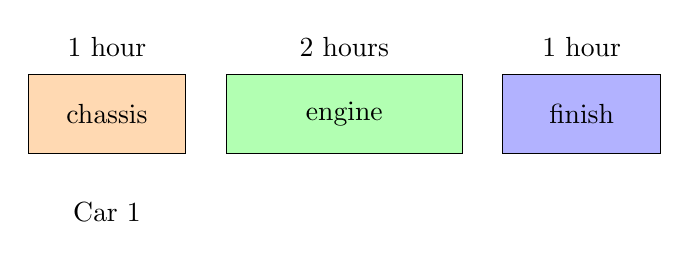
\begin{tikzpicture}[scale=0.9]
        \node[draw, fill=orange!30, minimum width=2cm, minimum height=1cm] (chassis) {chassis};
        \node[draw, fill=green!30, minimum width=3cm, minimum height=1cm, right=0.5cm of chassis] (engine) {engine};
        \node[draw, fill=blue!30, minimum width=2cm, minimum height=1cm, right=0.5cm of engine] (finish) {finish};
        
        \node[above=0.1cm of chassis] {1 hour};
        \node[above=0.1cm of engine] {2 hours};
        \node[above=0.1cm of finish] {1 hour};
        
        \node[below=0.5cm of chassis] {Car 1};
    \end{tikzpicture}
    
    \vspace{1cm}
    Time: 00:00
\end{frame}

%% Slide: Pipelined Car Assembly - Multiple Cars
\begin{frame}{Pipelined Car Assembly}
    \begin{itemize}
        \item Car 2 waited an hour after finishing station 1 for Car 1 to finish station 2
        \item Pipeline latency is 5 hours
        \item Pipeline throughput is one car every 2 hours
    \end{itemize}
    
    \centering
    
\begin{tikzpicture}[scale=0.8]
        % Simplified pipeline representation
        \node[draw, dashed, minimum width=10cm, minimum height=2cm] {
            Pipeline stages with multiple cars
        };
    \end{tikzpicture}
\end{frame}

%% Slide: Pipelining Instructions
\begin{frame}{Pipelining Instructions}
    \begin{columns}
        \column{0.5\textwidth}
        \textbf{Sequential Execution:}
        \begin{itemize}
            \item 8 ns per instruction
            \item Total: 24 ns for 3 instructions
        \end{itemize}
        
        \column{0.5\textwidth}
        \textbf{Pipelined Execution:}
        \begin{itemize}
            \item 2 ns per stage
            \item Total: 14 ns for 3 instructions
        \end{itemize}
    \end{columns}
    
    \vspace{0.5cm}
    \centering
    Program execution order:
    \begin{enumerate}
        \item \texttt{lw R1, 100(R0)}
        \item \texttt{lw R2, 200(R0)}
        \item \texttt{lw R3, 300(R0)}
    \end{enumerate}
    
    \textbf{Ideal speedup = Number of pipeline stages}
\end{frame}

%% Slide: Pipelining
\begin{frame}{Pipelining}
    \begin{itemize}
        \item Pipelining does not reduce the \textcolor{red}{latency} of single task, it increases the \textcolor{green}{throughput} of entire workload
        \item Potential speedup = Number of pipe stages
        \begin{itemize}
            \item Pipeline rate is limited by the slowest pipeline stage
            \item[$\Rightarrow$] Partition the pipe to many pipe stages
            \item[$\Rightarrow$] Make the longest pipe stage to be as short as possible
            \item[$\Rightarrow$] Balance the work in the pipe stages
        \end{itemize}
        \item Pipeline adds overhead (e.g., latches)
        \begin{itemize}
            \item Time to "fill" pipeline and time to "drain" it reduces speedup
            \item Stall for dependencies
            \item[$\Rightarrow$] Too many pipe-stages start to lose performance
        \end{itemize}
        \item IPC of an ideal pipelined machine is 1
        \begin{itemize}
            \item Every clock one instruction finishes
        \end{itemize}
    \end{itemize}
\end{frame}

%% Slide: Pipelined CPU
\begin{frame}{Pipelined CPU}
    \centering
    \begin{tikzpicture}[scale=0.7]
        % Placeholder for pipelined CPU diagram
        \node[draw, rectangle, minimum width=14cm, minimum height=7cm, dashed, align=center] {
            \Large Pipelined CPU Architecture\\
            \normalsize (Fetch $\rightarrow$ Decode $\rightarrow$ Execute $\rightarrow$ Memory $\rightarrow$ WB)\\
            \small with pipeline latches between stages
        };
    \end{tikzpicture}
\end{frame}

%% Slide: Structural Hazard
\begin{frame}{Structural Hazard}
    \begin{itemize}
        \item Different instructions using the same resource at the same time
        \item \textbf{Register File:}
        \begin{itemize}
            \item Accessed in 2 stages:
            \begin{itemize}
                \item Read during stage 2 (ID)
                \item Write during stage 5 (WB)
            \end{itemize}
            \item Solution: 2 read ports, 1 write port
        \end{itemize}
        \item \textbf{Memory:}
        \begin{itemize}
            \item Accessed in 2 stages:
            \begin{itemize}
                \item Instruction Fetch during stage 1 (IF)
                \item Data read/write during stage 4 (MEM)
            \end{itemize}
            \item Solution: separate instruction cache and data cache
        \end{itemize}
        \item Each functional unit can only be used \textcolor{green}{once} per instruction
        \item Each functional unit must be used at the \textcolor{green}{same} stage for all instructions
    \end{itemize}
\end{frame}

%% Slide: Pipeline Example
\begin{frame}{Pipeline Example: cycle 1}
    \begin{columns}
        \column{0.4\textwidth}
        \begin{tabular}{ll}
            0 & \texttt{lw R10,9(R1)}\\
            4 & \texttt{sub R11,R2,R3}\\
            8 & \texttt{and R12,R4,R5}\\
            12 & \texttt{or R13,R6,R7}
        \end{tabular}
        
        \column{0.6\textwidth}
        \centering
        PC = 0
        \vspace{0.5cm}
        
        \begin{tikzpicture}[scale=0.6]
            \node[draw, dashed, minimum width=8cm, minimum height=3cm, align=center] {
                Pipeline State Diagram\\
                (Cycle 1)
            };
        \end{tikzpicture}
    \end{columns}
\end{frame}

%% Slide: RAW Dependency
\begin{frame}{RAW Dependency}
    \begin{columns}
        \column{0.5\textwidth}
        Program execution order:
        \begin{enumerate}
            \item \texttt{sub R2, R1, R3}
            \item \texttt{and R12, \textcolor{red}{R2}, R5}
            \item \texttt{or R13, R6, \textcolor{red}{R2}}
            \item \texttt{add R14, \textcolor{red}{R2}, \textcolor{red}{R2}}
            \item \texttt{sw R15, 100(\textcolor{red}{R2})}
        \end{enumerate}
        
        \column{0.5\textwidth}
        \centering
        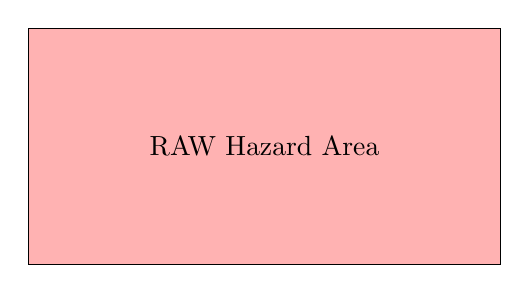
\begin{tikzpicture}[scale=0.5]
            % Pipeline stages showing dependency
            \node[draw, fill=red!30, minimum width=6cm, minimum height=3cm] {
                RAW Hazard Area
            };
        \end{tikzpicture}
    \end{columns}
\end{frame}

%% Slide: Using Bypass to Solve RAW Dependency
\begin{frame}{Using Bypass to Solve RAW Dependency}
    \begin{itemize}
        \item Bypass result directly from EXE output to EXE input
        \item No stall needed when bypass is possible
        \item Hardware forwards data from:
        \begin{itemize}
            \item EXE/MEM pipeline register
            \item MEM/WB pipeline register
        \end{itemize}
    \end{itemize}
    
    \centering
    \begin{tikzpicture}[scale=0.7]
        \node[draw, dashed, minimum width=10cm, minimum height=4cm] {
            Bypass/Forwarding Hardware Diagram
        };
    \end{tikzpicture}
\end{frame}

%% Slide: Bypass Control
\begin{frame}[fragile]{Bypass Control}
    \textbf{L3\_reg\_wr = L3.RegWrite and (L3.opcode != lw)}
    
    \vspace{0.3cm}
    \textbf{Forwarding from EXE (L3):}
    \begin{itemize}
        \item \small if (L3\_reg\_wr and (L3.dst == L2.src1)) ALUSelA = 1
        \item \small if (L3\_reg\_wr and (L3.dst == L2.src2)) ALUSelB = 1
    \end{itemize}
    
    \vspace{0.3cm}
    \textbf{Forwarding from MEM (L4):}
    \begin{itemize}
        \item \small if (L4.RegWrite and ((not L3\_reg\_wr) or (L3.dst $\neq$ L2.src1))\\
              and (L4.dst = L2.src1)) ALUSelA = 2
        \item \small if (L4.RegWrite and ((not L3\_reg\_wr) or (L3.dst $\neq$ L2.src2))\\
              and (L4.dst = L2.src2)) ALUSelB = 2
    \end{itemize}
\end{frame}

%% Slide: Register File Split
\begin{frame}{Register File Split}
    \begin{itemize}
        \item Register file is written during first half of the cycle
        \item Register file is read during second half of the cycle
        \item[$\Rightarrow$] Register file is written before it is read $\Rightarrow$ returns the correct data
    \end{itemize}
    
    \centering
    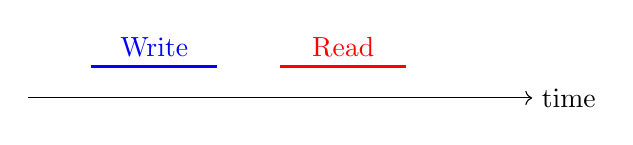
\begin{tikzpicture}[scale=0.8]
        % Timeline showing register file operations
        \draw[->] (0,0) -- (8,0) node[right] {time};
        \draw[thick, blue] (1,0.5) -- (3,0.5) node[midway, above] {Write};
        \draw[thick, red] (4,0.5) -- (6,0.5) node[midway, above] {Read};
    \end{tikzpicture}
\end{frame}

%% Slide: Can't Always Bypass
\begin{frame}{Can't Always Bypass}
    \begin{itemize}
        \item Load word can still cause a hazard
        \begin{itemize}
            \item An instruction tries to read a register following a load instruction that writes to the same register
        \end{itemize}
        \item A hazard detection unit is needed to "stall" the load instruction
    \end{itemize}
    
    Program execution order:
    \begin{enumerate}
        \item \texttt{lw \textcolor{red}{R2}, 30(R1)}
        \item \texttt{and R12, \textcolor{red}{R2}, R5}
        \item \texttt{or R13, R6, \textcolor{red}{R2}}
        \item \texttt{add R14, \textcolor{red}{R2}, \textcolor{red}{R2}}
        \item \texttt{sw R15, 100(\textcolor{red}{R2})}
    \end{enumerate}
\end{frame}

%% Slide: Stall If Cannot Bypass
\begin{frame}[fragile]{Stall If Cannot Bypass}
    \begin{verbatim}
if (L2.RegWrite and (L2.opcode == lw) and 
    ((L2.dst == L1.src1) or (L2.dst == L1.src2))) 
then stall
    \end{verbatim}
    
    \vspace{0.5cm}
    \begin{itemize}
        \item De-assert the enable to the L1 latch, and to the IP
        \begin{itemize}
            \item The dependent instruction (and) stays another cycle in L1
        \end{itemize}
        \item Issue a NOP into the L2 latch (instead of the stalled inst.)
        \item Allow the stalling instruction (lw) to move on
    \end{itemize}
    
    \centering
    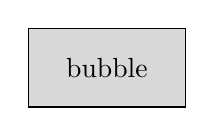
\begin{tikzpicture}[scale=0.6]
        \node[draw, fill=gray!30, minimum width=2cm, minimum height=1cm] {bubble};
    \end{tikzpicture}
\end{frame}

%% Slide: Software Scheduling to Avoid Load Hazards
\begin{frame}[fragile]{Software Scheduling to Avoid Load Hazards}
    Example: code for (assume all variables are in memory):
    \begin{center}
        \texttt{a = b + c;}\\
        \texttt{d = e - f;}
    \end{center}
    
    \begin{columns}
        \column{0.5\textwidth}
        \textbf{Slow code:}
        \begin{verbatim}
LW   Rb,b
LW   Rc,c
Stall
ADD  Ra,Rb,Rc
SW   a,Ra
LW   Re,e
LW   Rf,f
Stall
SUB  Rd,Re,Rf
SW   d,Rd
        \end{verbatim}
        
        \column{0.5\textwidth}
        \textbf{Fast code:}
        \begin{verbatim}
LW   Rb,b
LW   Rc,c
LW   Re,e
ADD  Ra,Rb,Rc
LW   Rf,f
SW   a,Ra
SUB  Rd,Re,Rf
SW   d,Rd
        \end{verbatim}
    \end{columns}
    
    \vspace{0.5cm}
    \centering
    \textit{Instruction order can be changed as long as the correctness is kept}
\end{frame}

\begin{frame}[label=control-hazard]{Control Hazard on Branches}
    \centering
    \drawPipelineDiagram
\end{frame}

%% Slide: Control Hazard on Branches - With Annotations
\begin{frame}[label=control-hazard-annotated]{Control Hazard on Branches}
    \centering
    \drawPipelineDiagram
    
    % Add annotations specific to this slide
    \begin{tikzpicture}[remember picture, overlay]
        % Add blue numbers for PC values
        \node[blue, font=\footnotesize\bfseries] at ($(current page.center) + (-6.4,-1.2)$) {8};
        \node[blue, font=\footnotesize\bfseries] at ($(current page.center) + (-3.7,1.4)$) {12};
        \node[blue, font=\footnotesize\bfseries] at ($(current page.center) + (-1.4,1.4)$) {8};
        \node[blue, font=\footnotesize\bfseries] at ($(current page.center) + (1.1,1.4)$) {4};
        
        % Add instruction labels in latches
        \node[font=\footnotesize\bfseries] at ($(current page.center) + (-3.05,-0.3)$) {jcc};
        \node[font=\footnotesize\bfseries] at ($(current page.center) + (-0.7,-0.3)$) {or};
        
        % Add orange highlight around certain paths
        \draw[orange!50, very thick, rounded corners] ($(current page.center) + (-7.0,0.9)$) rectangle ($(current page.center) + (6.4,3.1)$);
        
        % Add green highlight for decode stage
        \draw[green!50, very thick, rounded corners] ($(current page.center) + (-3.7,-1.5)$) rectangle ($(current page.center) + (-1.8,1.3)$);
        
        % Add text annotations at bottom
        \node[font=\footnotesize, align=left] at ($(current page.center) + (0,-3.0)$) {
            \texttt{jcc target; if cond then PC $\leftarrow$ target}
        };
        \node[font=\footnotesize, align=left, text=green!70!black] at ($(current page.center) + (0,-3.5)$) {
            $\diamond$ The target is saved in the instruction relative to the address of the fall-through instruction
        };
        \node[font=\footnotesize, align=left, text=green!70!black] at ($(current page.center) + (0,-4.0)$) {
            $\diamond$ Most conditional jumps are short (if and loop) $\Rightarrow$ save bits in the instruction encoding
        };
    \end{tikzpicture}
\end{frame}

%% Slide: Control Hazard: Stall
\begin{frame}{Control Hazard: Stall}
    \begin{itemize}
        \item Stall pipe when branch is encountered until resolved
        \item Stall impact: assumptions
        \begin{itemize}
            \item CPI = 1
            \item 20\% of instructions are branches
            \item Stall 3 cycles on every branch
            \item[$\Rightarrow$] CPI\textsubscript{new} = 1 + 0.2 × 3 = 1.6
        \end{itemize}
    \end{itemize}
    
    \vspace{0.5cm}
    \centering
    (CPI\textsubscript{new} = CPI\textsubscript{Ideal} + avg. stall cycles / instr.)
    
    \vspace{0.5cm}
    \textbf{We lose 60\% of the performance}
\end{frame}

%% Slide: Control Hazard: Stall  
\begin{frame}{Control Hazard: Stall}
    \begin{itemize}
        \item Stall pipe when branch is encountered until resolved
        \item Stall impact: assumptions
        \begin{itemize}
            \item CPI = 1
            \item 20\% of instructions are branches
            \item Stall 3 cycles on every branch
            \item[$\Rightarrow$] CPI\textsubscript{new} = 1 + 0.2 × 3 = 1.6
        \end{itemize}
    \end{itemize}
    
    \vspace{0.5cm}
    \centering
    (CPI\textsubscript{new} = CPI\textsubscript{Ideal} + avg. stall cycles / instr.)
    
    \vspace{0.5cm}
    \textbf{We lose 60\% of the performance}
\end{frame}

%% Slide: Control Hazard: Predict Not Taken
\begin{frame}{Control Hazard: Predict Not Taken}
    \begin{itemize}
        \item Execute instructions from the fall-through (not-taken) path
        \begin{itemize}
            \item As if there is no branch
            \item If the branch is not-taken ($\sim50\%$), no penalty is paid
        \end{itemize}
        \item If branch actually taken
        \begin{itemize}
            \item Flush the fall-through path instructions before they change the machine state (memory / registers)
            \item Fetch the instructions from the correct (taken) path
        \end{itemize}
        \item Assuming 20\% of instructions are branches and $\sim50\%$ branches not taken on average
        \begin{itemize}
            \item CPI\textsubscript{new} = 1 + (0.2 × 0.5) × 3 = 1.3
        \end{itemize}
    \end{itemize}
\end{frame}

%% Slide: Dynamic Branch Prediction
\begin{frame}{Dynamic Branch Prediction}
    \begin{itemize}
        \item \textbf{Branch Target Buffer} (BTB) that predicts (at fetch)
        \begin{itemize}
            \item[$\diamond$] Instruction is a branch
            \item[$\diamond$] Branch taken / not-taken
            \item[$\diamond$] Taken branch target
        \end{itemize}
    \end{itemize}
    
    \vspace{0.3cm}
    
    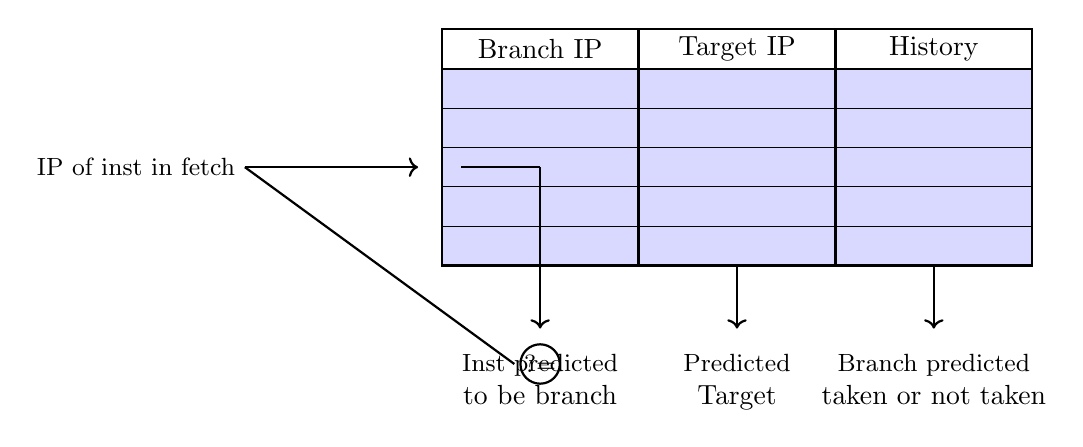
\begin{tikzpicture}[scale=1]
        % Draw the BTB table with light blue fill for data area
        \fill[blue!15] (0,0) rectangle (7.5,2.5);
        
        % Draw outer border
        \draw[thick] (0,0) rectangle (7.5,3);
        
        % Column dividers
        \draw[thick] (2.5,0) -- (2.5,3);
        \draw[thick] (5,0) -- (5,3);
        
        % Header row separator
        \draw[thick] (0,2.5) -- (7.5,2.5);
        
        % Data row lines (4 rows shown)
        \draw (0,2) -- (7.5,2);
        \draw (0,1.5) -- (7.5,1.5);
        \draw (0,1) -- (7.5,1);
        \draw (0,0.5) -- (7.5,0.5);
        
        % Header text
        \node at (1.25,2.75) {Branch IP};
        \node at (3.75,2.75) {Target IP};
        \node at (6.25,2.75) {History};
        
        % Arrow from "IP of inst in fetch" to comparison circle
        \draw[->,thick] (-2.5,1.25) -- (-0.3,1.25);
        \node[left] (ip) at (-2.5,1.25) {\small IP of inst in fetch};
        
        % Comparison circle positioned between arrow and Branch IP column
        \draw[thick,fill=white] (1.25,-1.25) circle (0.25);
        \node (qmark) at (1.25,-1.25) {\small ?=};
        \draw[thick] (ip.east) -- (qmark.west);
        
        % Connect comparison to Branch IP column (horizontal then down)
        \draw[thick] (0.25,1.25) -- (1.25,1.25);
        \draw[->,thick] (1.25,1.25) -- (1.25,0) -- (1.25,-0.8);
        
        % Arrow from Target IP column straight down
        \draw[->,thick] (3.75,0) -- (3.75,-0.8);
        
        % Arrow from History column straight down
        \draw[->,thick] (6.25,0) -- (6.25,-0.8);
        
        % Output labels
        \node[below,align=center] at (1.25,-1) {\small Inst predicted\\to be branch};
        \node[below,align=center] at (3.75,-1) {\small Predicted\\Target};
        \node[below,align=center] at (6.25,-1) {\small Branch predicted\\taken or not taken};
    \end{tikzpicture}
    
    \vspace{0.4cm}
    
    \begin{itemize}
        \item BTB allocated at execute -- after all branch info is known
        \item BTB is looked up at instruction fetch
    \end{itemize}
\end{frame}


%% Slide: BTB
\begin{frame}{BTB}
    \begin{itemize}
        \item \textbf{Allocation} – at Decode / EXE
        \begin{itemize}
            \item Allocate instructions identified as branches (after decode)
            \item Not taken branches need not be allocated
            \item BTB miss implicitly predicts not-taken
        \end{itemize}
        \item \textbf{Prediction} – at Fetch
        \begin{itemize}
            \item BTB lookup is done parallel to IC lookup
            \item BTB provides:
            \begin{itemize}
                \item Indication that the instruction is a branch (BTB hits)
                \item Branch predicted target
                \item Branch predicted direction
                \item Branch predicted type (e.g., conditional, unconditional)
            \end{itemize}
        \end{itemize}
        \item \textbf{Update} (when branch outcome is known – at EXE)
        \begin{itemize}
            \item Branch target
            \item Branch history (taken / not-taken)
        \end{itemize}
    \end{itemize}
\end{frame}

%% Slide: BTB (cont.)
\begin{frame}{BTB (cont.)}
    \begin{itemize}
        \item \textbf{Wrong prediction}
        \begin{itemize}
            \item Predict not-taken, actual taken
            \item Predict taken, actual not-taken, or actual taken but wrong target
        \end{itemize}
        \item \textbf{In case of wrong prediction – flush the pipeline}
        \begin{itemize}
            \item Reset latches (same as making all instructions to be NOPs)
            \item Select the PC source to be from the correct path
            \item Need get the fall-through with the branch
            \item Start fetching instruction from correct path
        \end{itemize}
        \item \textbf{Assuming P\% correct prediction rate}
        \begin{itemize}
            \item CPI\textsubscript{new} = 1 + (0.2 × (1-P)) × 3
            \item For example, if P=0.7
            \item CPI\textsubscript{new} = 1 + (0.2 × 0.3) × 3 = 1.18
        \end{itemize}
    \end{itemize}
\end{frame}

%% Slide: Adding a BTB to the Pipeline
\begin{frame}{Adding a BTB to the Pipeline}
    \centering
    \begin{tikzpicture}[scale=0.7]
        % Placeholder for BTB pipeline integration diagram
        \node[draw, rectangle, minimum width=14cm, minimum height=7cm, dashed, align=center] {
            \Large BTB Integration with Pipeline\\
            \normalsize BTB lookup parallel with I-cache lookup\\
            \small Predicted target and direction available at Fetch
        };
    \end{tikzpicture}
\end{frame}

%% Slide: Using The BTB
\begin{frame}{Using The BTB}
    \centering
    \tiny
    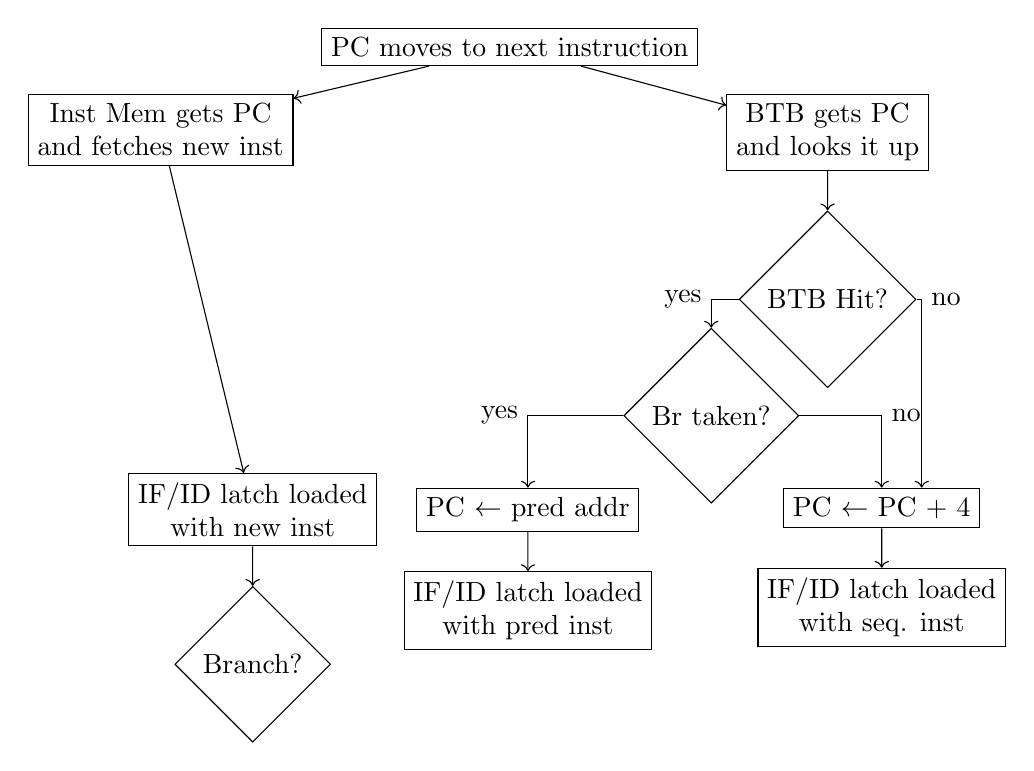
\begin{tikzpicture}[scale=0.8, node distance=0.5cm]
        % Flowchart for BTB usage
        \node[draw, rectangle] (pc) {PC moves to next instruction};
        \node[draw, rectangle, below left=of pc, align=center] (imem) {Inst Mem gets PC\\and fetches new inst};
        \node[draw, rectangle, below right=of pc, align=center] (btb) {BTB gets PC\\and looks it up};
        \node[draw, diamond, below=of btb] (hit) {BTB Hit?};
        \node[draw, diamond, below left=of hit] (taken) {Br taken?};
        \node[draw, rectangle, below left=of taken] (pred) {PC $\leftarrow$ pred addr};
        \node[draw, rectangle, below right=of taken] (inc) {PC $\leftarrow$ PC + 4};
        \node[draw, rectangle, below=of pred, align=center] (predinst) {IF/ID latch loaded\\with pred inst};
        \node[draw, rectangle, below=of inc, align=center] (seqinst) {IF/ID latch loaded\\with seq. inst};
        \node[draw, rectangle, left=of pred, align=center] (new) {IF/ID latch loaded\\with new inst};
        \node[draw, diamond, below=of new, align=center] (branch) {Branch?};
        
        \draw[->] (pc) -- (imem);
        \draw[->] (pc) -- (btb);
        \draw[->] (btb) -- (hit);
        \draw[->] (hit) -| node[left] {yes} (taken);
        \draw[->] (hit) -| node[right] {no} ([xshift=6.5cm]inc);
        \draw[->] (taken.west) -| node[left] {yes} (pred);
        \draw[->] (taken) -| node[right] {no} (inc);
        \draw[->] (pred) -- (predinst);
        \draw[->] (inc) -- (seqinst);
        \draw[->] (imem) -- (new);
        \draw[->] (new) -- (branch);
    \end{tikzpicture}
\end{frame}

%% Slide: Using The BTB (cont.)
\begin{frame}{Using The BTB (cont.)}
    \centering
    \tiny
    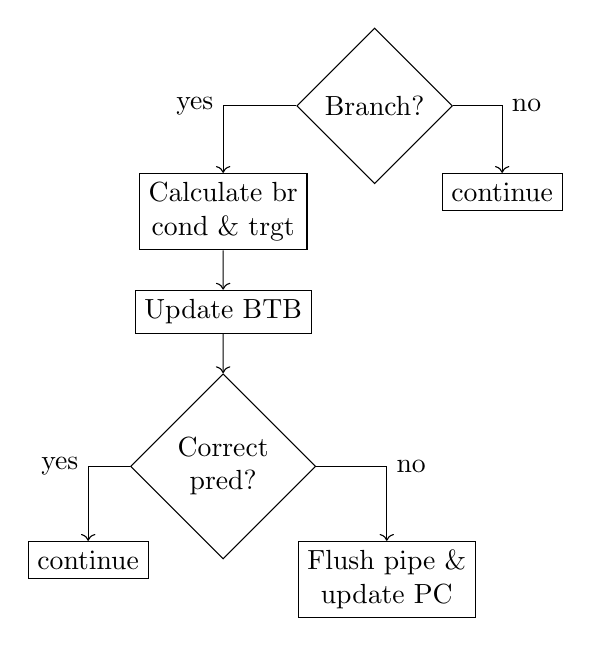
\begin{tikzpicture}[scale=0.8, node distance=0.5cm]
        % Continuation of BTB flowchart
        \node[draw, diamond] (branch) {Branch?};
        \node[draw, rectangle, below left=of branch, align=center] (calc) {Calculate br\\cond \& trgt};
        \node[draw, rectangle, below right=of branch] (continue1) {continue};
        \node[draw, rectangle, below=of calc] (update) {Update BTB};
        \node[draw, diamond, below=of update, align=center] (correct) {Correct\\pred?};
        \node[draw, rectangle, below right=of correct, align=center] (flush) {Flush pipe \&\\update PC};
        \node[draw, rectangle, below left=of correct] (continue2) {continue};
        
        \draw[->] (branch) -| node[left] {yes} (calc);
        \draw[->] (branch) -| node[right] {no} (continue1);
        \draw[->] (calc) -- (update);
        \draw[->] (update) -- (correct);
        \draw[->] (correct) -| node[right] {no} (flush);
        \draw[->] (correct) -| node[left] {yes} (continue2);
    \end{tikzpicture}
\end{frame}

\end{document}